\documentclass[english]{RMcv}
%
\hypersetup{%
    hidelinks,%
    colorlinks=false,%
    pdfauthor={Riccardo Milani},%
    pdftitle={Milani's resume},%
    pdfdisplaydoctitle=true,%
    %pdfsubject={CV},
    pdfkeywords={resume,CV},%
    %pdfpagemode=FullScreen,%
    %pdfmenubar=false,%
    %pdftoolbar=false,%
    pdflang=en-US,%
    pdfcreator=LaTeX,%
}

%\renewcommand\intracvevent{4pt} % Spacing between a cvevent and the previous object. Default: 6pt
%\renewcommand\intercvevent{4pt} % Spacing between first line and bullet point of a cvevent. Default: 6pt

\title{CV - Eng}

\newif\ifcvtitle
\newif\ifcvsubtitle
\cvtitlefalse
\cvsubtitlefalse

%============================================================================%
%
%
%
%  DOCUMENT CONTENT
%
%
%
%============================================================================%
\begin{document}

%---------------------------------------------------------------------------------------
%  TITLE HEADLINE
%----------------------------------------------------------------------------------------
\vspace{-20.55pt}

\cvhead{Resume}

\vspace{2px}
\center{%
 \ifcvtitle{Mathematical Engineer $\cdot$} \fi%
 Italian, French $\cdot$ %\faFlag~
 15/01/1991 $\cdot$ %
 Paris $\cdot$ %
 \href{mailto:ricc.milani@gmail.com}{\textcolor{sectcol}{\textbf{ricc.milani@gmail.com}}} $\cdot$ %\faEnvelope
 {+33 7 83 93 34 47} $\cdot$ %\faPhone or \faMobilePhone\footnotesize
 \textcolor{sectcol}{\faLinkedinSquare\href{https://www.linkedin.com/in/milanir/?locale=en_US}{\bfseries/in/milanir}} $\cdot$ %
 \faGithub\href{https://github.com/RiMillo}{/RiMillo}% $\cdot$ %
}
\vspace{2px}
\center{\huge{\textbf{\textcolor{sectcol}{%
% Title
\ifcvtitle%
  PhD in Applied Mathematics / CFD%
\else%
  PhD, Mathematical Engineer%
\fi
}}}}%
%\vspace{-2px}
% ================
% Subtitle
\ifcvsubtitle%
  \center{\large{\textcolor{bgcol}{Starting summer/fall 2017}}}%
\else%
  \vspace*{2px}
\fi
\vspace*{4px}%
% ================
\vspace{4px}%
%
%----------------------------------------------------------------------------------------
%  HEADER IMAGE
%----------------------------------------------------------------------------------------

%\begin{figure}[H]
%\begin{flushright}
  %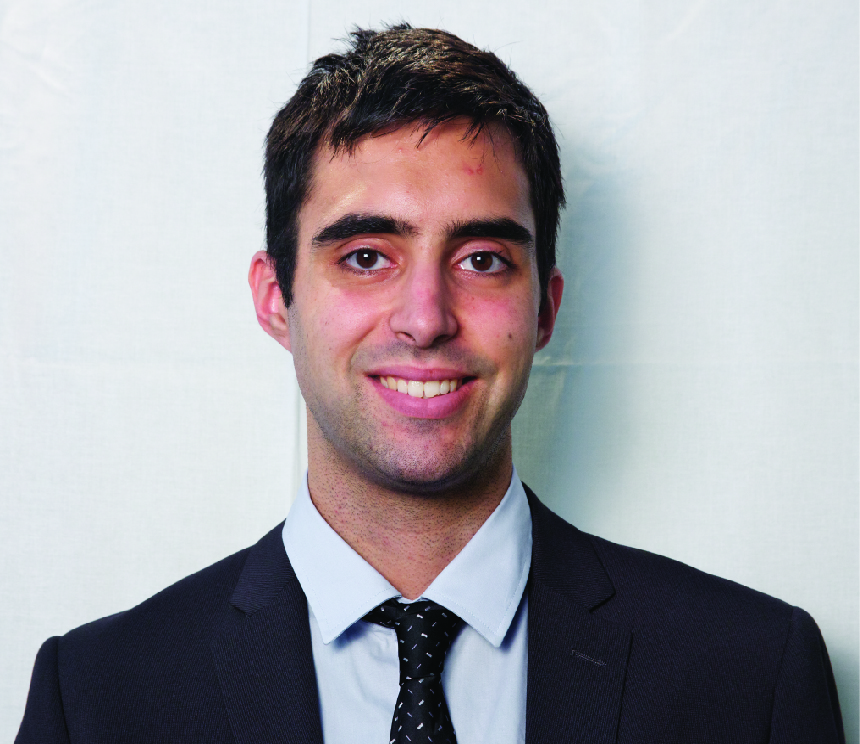
\includegraphics[trim= 320 130 460 210,clip,width=0.2\linewidth]{Foto_Smart.jpg}  %trimming relative to image size!
    %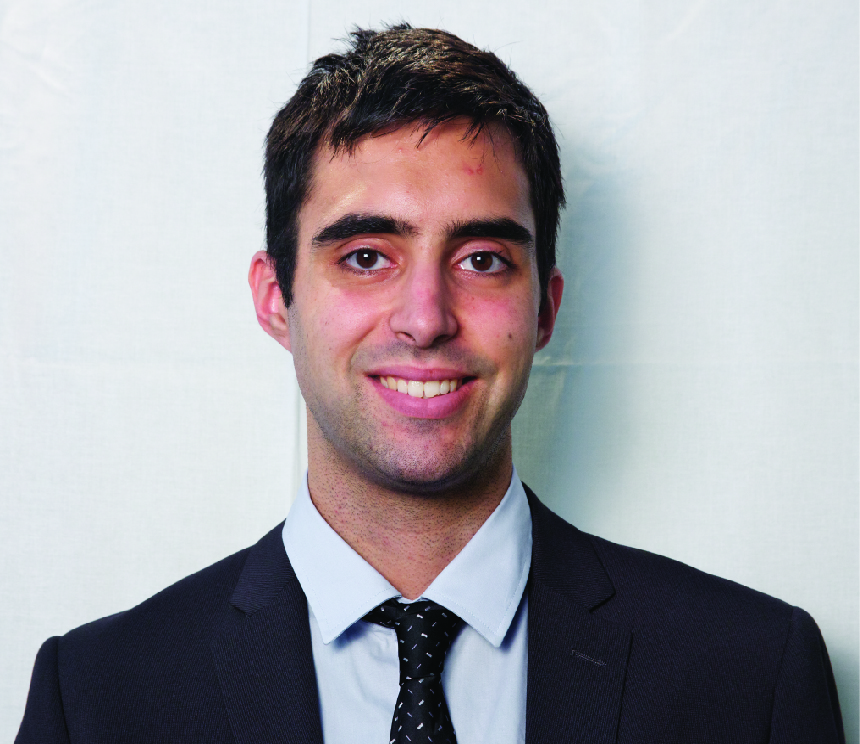
\includegraphics[width=0.2\linewidth]{Foto_Smart.jpg}
%\end{flushright}
%\end{figure}

%---------------------------------------------------------------------------------------
%  QR CODE (optional)
%----------------------------------------------------------------------------------------
%\vspace{-136pt}
%\hspace{0.75\linewidth}
%
\includegraphics[width=103pt]{qrcode}
%\normalsize
%\vspace{88pt}

%---------------------------------------------------------------------------------------
%  META SECTION
%----------------------------------------------------------------------------------------

%\vspace{-114pt}

%\metasection{Status:}{M.Sc. Digital Media, IT Consultant at We4IT Bremen}
%\metasection{Fields:}{Project Management, Software Development, Scrum, Usability}
%\metasection{Prefers:}{JS, Java, XPages, Flex / AIR, Processing, Git, Eclipse}
%\metasection{Activities:}{Global Game Jam, Sound Engineering, Blender, Martial Arts}

%\vspace{6pt}

%---------------------------------------------------------------------------------------
%  SUMMARAY (optional)
%----------------------------------------------------------------------------------------

%\cvsection{Summary}\\
%Digital media graduate with four years project experience in the field of technology based assessment. Specialized in development of test-scenario engines and innovative, rich media item formats. Master studies focused on teams from different disciplines and cultural backgrounds on solutions for complex problems.  Prior knowledge has been collected in he field of usability / accessibility during bachelor studies.\\

%============================================================================%
%
%  CV SECTIONS AND EVENTS (MAIN CONTENT)
%
%============================================================================%

%---------------------------------------------------------------------------------------
%  EDUCATION SECTION
%--------------------------------------------------------------------------------------
\cvsection{Education}

\cvevent{since 2021}%
        {Postdoctoral researcher}%
        {CEREA - \'Ecole des Ponts ParisTech}%
        {\href{https://sciences2024.polytechnique.fr/}{\textsc{Sciences}\textsuperscript{2024}} - the physics of sports}%
        {Archery: Simulation of arrow flight under real-life conditions}

\cvevent{2017 - 2020}%
        {PhD Student in Applied Mathematics}%
        {\'Ecole des Ponts ParisTech, INRIA, EDF R\&D}%
        {\href{https://tel.archives-ouvertes.fr/tel-03080530}{\emph{Compatible Discrete Operator} schemes for the unsteady incompressible Navier–Stokes equations}}%
        {Advisors: Ern Alexandre (ENPC, INRIA) and Bonelle J\'er\^ome (EDF R\&D)}

\cvevent{2015 - 2017}%
        {MSc in Mathematical Engineering}%
        {Politecnico di Milano}%
        {\href{https://www.politesi.polimi.it/handle/10589/133692}{\emph{Laurea Magistrale}} in Mathematical Engineering, specialization: Applied Mathematics \& Computer Sciences}{Score: 110 and honors/110}

%\textcolor{softcol}{\hrule}

%
\cvevent{2013 - 2017}%
        {Cycle of \textit{Polytechnicien} Engineer}%
        {\'Ecole polytechnique}%
        {Education cycle equivalent to BSc and MSc}{Specialization: Applied Mathematics - PDEs}

%\textcolor{softcol}{\hrule}

%
\cvevent{2010 - 2015}%
        {BSc in Mathematical Engineering}%
        {Politecnico di Milano}%
        {\emph{Laurea Triennale} in Mathematical Engineering. Score: 110 and honors/110}{Awarded "Best freshman" (2010) after the results of the entry test and first semester exams}

%---------------------------------------------------------------------------------------
%  EXPERIENCE
%----------------------------------------------------------------------------------------
\cvsection{Experience}

%
\cvevent{09/'16-02/'17}%
        {Research Internship, 6 months}%
        {EDF R\&D, Chatou}%
        {\href{https://www.politesi.polimi.it/handle/10589/133692}{Development and numerical analysis of a 3D HHO method for anisotropic diffusion}}%
        {Integration within the industrial code \cs{} (\texttt{C}); parallelization by OpenMP}

%\textcolor{softcol}{\hrule}

%
\cvevent{03-08/2015}{Research Internship, 5 months}%
        {US ESI R\&D, San Diego}%
        {First steps into the development of a new method for a fast computation of the vibro-acoustic response of a system}%
        {Validations against software simulations}

%\textcolor{softcol}{\hrule}

%
%\cvevent{08/2014}%
        %{Summer Internship}%
        %{VTB Bank, Irkutsk}%
        %{Foreign Exchange Control Group}{Support in the preparation and final validation of files about international contracts, records management}

\vspace{12pt}
\begin{minipage}{.48\linewidth}
\begin{flushleft}
\cvsubsection{Programming skills}
\vspace{6pt}
\begin{tabular*}{1\linewidth}{l l}
&     \larrow{bgcol} \textbf{Good knowledge}: \texttt{C}/\texttt{C++}, OpenMP, MPI, \href{https://github.com/RiMillo/LaTeX_tips}{\LaTeX},\\[3pt]
&       Unix systems, MATLAB, Git/SVN, \href{https://www.code-saturne.org/cms/}{\cs{}}, Office\\[3pt]
&     \larrow{bgcol} \textbf{Basic knowledge}: Python, shell scripting, Fortran,\\[3pt]
&       FreeFem\texttt{++}, SALOME, Java, R\\[3pt]
  \end{tabular*}
\end{flushleft}
\end{minipage}
\hfill
\begin{minipage}{.48\linewidth}
\begin{flushright}
\cvsubsection{Languages}
\vspace{6pt}
\begin{tabular*}{1\linewidth}{l l l}
&     \larrow{bgcol} \textbf{Italian}: &Native\\[3pt]
&     \larrow{bgcol} \textbf{English}: &Fluent, FCE certificate, B2\\[3pt]
&     \larrow{bgcol} \textbf{French}:  &Fluent, TCF certificate, C1\\[3pt]
&     \larrow{bgcol} \textbf{Russian}: &Conversational level\\[3pt]
\end{tabular*}
\end{flushright}
\end{minipage}

\bigskip

\begin{minipage}{.48\linewidth}
\begin{flushleft}
\cvsubsection{Extracurricular activities}
\vspace{6pt}
\begin{tabular*}{1\linewidth}{l l}
&     \larrow{bgcol} Head of a 40-student dormitory ('15) \\[3pt]
&     \larrow{bgcol} General-treasurer of \href{https://www.aim-mate.it/en/}{AIM} ('16)\\[3pt]
&     \larrow{bgcol} PhD-students representative for EDF-MFEE ('18-'20)\\[3pt]
&     \larrow{bgcol} Running (Paris marathon '19)\\[3pt]
\end{tabular*}
\end{flushleft}
\end{minipage}
\hfill
\begin{minipage}{.48\linewidth}
\begin{flushright}
\cvsubsection{Volunteering and other Interests}
\vspace{6pt}
\begin{tabular*}{1\linewidth}{l l}
&     \larrow{bgcol} Summer work camps (Kenya '10, '11; Rwanda '17')\\[3pt]
&     \larrow{bgcol} Active member of Smileland, which backs \\[3pt]
&       an orphans village in Congo\\[3pt]
&     \larrow{bgcol} Italian classes for refugees ('15)\\[3pt]
\end{tabular*}
\end{flushright}
\end{minipage}




%-------------------------------------------------------------------------------------------------
%  ARTIFICIAL FOOTER (fancy footer cannot exceed linewidth)
%--------------------------------------------------------------------------------------------------

\null
\vspace*{\fill}
%\hspace{-0.25\linewidth}\colorbox{bgcol}{\makebox[1.5\linewidth][c]{\mystrut \small \textcolor{white}{www.jankuester.com} $\cdot$ \textcolor{white}{github.com/jankapunkt}}}




%============================================================================%
%
%
%
%  DOCUMENT END
%
%
%
%============================================================================%
\end{document}
